\subsubsection{Testbench và Kết quả mô phỏng Khối Bộ nhớ (Memory)}

\textbf{a. Mô tả kịch bản kiểm chứng (Testbench)} \\
Môi trường mô phỏng khối Memory được thiết lập để kiểm tra khả năng lưu trữ dữ liệu và tính đúng đắn của cổng giao tiếp song hướng (\textit{bidirectional port}). Các kịch bản kiểm thử bao gồm:
\begin{itemize}
    \item \textbf{Khởi tạo hệ thống}: Thiết lập các giá trị ban đầu và kiểm tra trạng thái trở kháng cao (\texttt{Hi-Z}) của bus dữ liệu khi không có lệnh đọc/ghi.
    \item \textbf{Thao tác Ghi (Write)}: Thực hiện ghi các giá trị dữ liệu cụ thể vào các địa chỉ khác nhau trong RAM tại cạnh lên của xung clock để kiểm tra tính đồng bộ.
    \item \textbf{Thao tác Đọc (Read)}: Truy xuất dữ liệu từ các địa chỉ đã ghi trước đó để đối chiếu tính toàn vẹn của dữ liệu.
    \item \textbf{Kiểm tra tách biệt Đọc/Ghi}: Đảm bảo rằng bus dữ liệu không bị xung đột khi chuyển đổi giữa chế độ đọc và ghi (sử dụng trạng thái trở kháng cao \texttt{32'bz}).
\end{itemize}

\textbf{b. Mã nguồn Testbench (Verilog)}
\begin{lstlisting}[language=Verilog, caption={Ma nguon Testbench kiem tra khoi Bo nho (Memory)}]
`timescale 1ns / 1ps

module tb_memory();

    reg          clk;
    reg  [31:0]  addr;
    reg          rd;
    reg          wr;
    wire [31:0]  data;

    reg  [31:0]  data_reg;
    assign data = (wr && !rd) ? data_reg : 32'bz;

    memory uut (
        .clk(clk),
        .addr(addr),
        .rd(rd),
        .wr(wr),
        .data(data)
    );

    always #5 clk = ~clk;

    initial begin
        clk = 0; addr = 0; rd = 0; wr = 0; data_reg = 0;

        $display("------------");
        $display(" Time|rd|wr|addr|data(hex)");
        $display("------------");
        
        // --- DONG QUAN TRONG NHAT: Monitor de in so lieu ra Console ---
        $monitor("%10t|%b|%b|%h|%h", $time, rd, wr, addr, data);

        // 1. Ghi du lieu vao o nho 0x01
        #10; addr = 32'h01; data_reg = 32'hABCD_1234; wr = 1; rd = 0;
        #10; wr = 0; 

        // 2. Ghi du lieu vao o nho 0x02
        #10; addr = 32'h02; data_reg = 32'h5555_AAAA; wr = 1;
        #10; wr = 0;

        // 3. Doc du lieu tu o nho 0x01
        #10; addr = 32'h01; rd = 1; wr = 0;
        #10; 
        
        // 4. Doc du lieu tu o nho 0x02
        #10; addr = 32'h02;
        #10;

        // 5. Trang thai nghi
        #10; rd = 0; wr = 0;
        #10;

        $display("------------");
        $display("Hoan thanh mo phong Memory!");
        $finish;
    end
endmodule
\end{lstlisting}

\textbf{c. Sơ đồ mạch RTL (RTL Schematic)} \\
Sơ đồ tổng hợp khối Memory thể hiện cấu trúc của mảng lưu trữ RAM và khối logic điều khiển cổng đệm ba trạng thái (\textit{Tri-state buffer}) phục vụ cho chân giao tiếp \texttt{inout}.

\begin{figure}[H]
    \centering
    % Thay 'sodomemory.png' bang ten file anh thuc te cua ban
    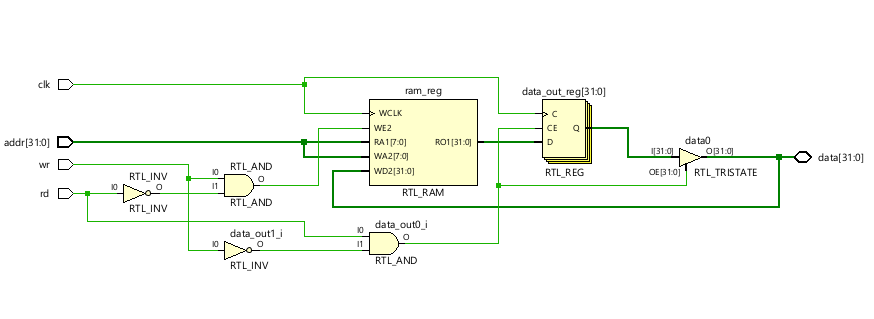
\includegraphics[width=0.8\textwidth]{sodomem.png} 
    \caption{Sơ đồ mạch logic (RTL Schematic) của khối Memory}
    \label{fig:mem_rtl}
\end{figure}

\textbf{d. Kết quả mô phỏng (Waveform)} \\
Sự thay đổi của bus dữ liệu khi thực hiện các thao tác ghi và đọc được thể hiện chi tiết trên giản đồ thời gian, đặc biệt là trạng thái trở kháng cao khi không có lệnh.

\begin{figure}[H]
    \centering
    % Thay 'wavememory.png' bang ten file anh thuc te cua ban
    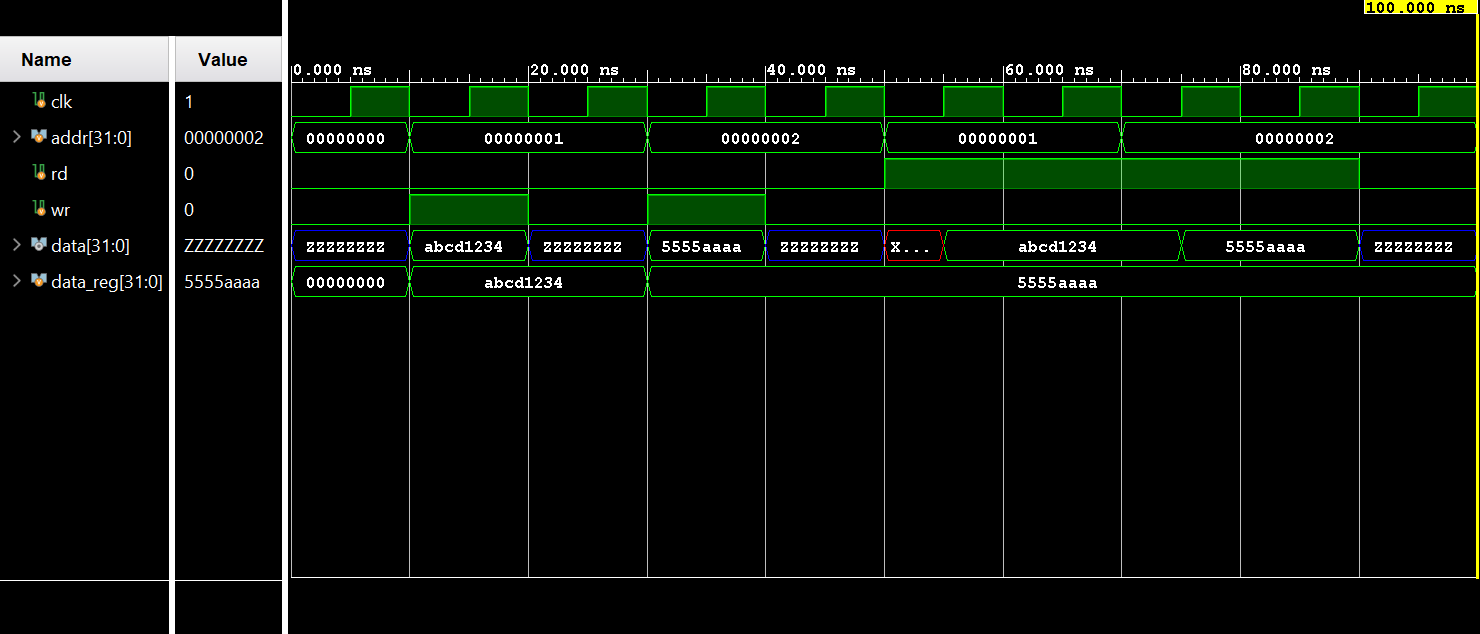
\includegraphics[width=\textwidth]{wavemem.png} 
    \caption{Giản đồ thời gian (Waveform) mô phỏng khối Memory}
    \label{fig:mem_wave}
\end{figure}

\textbf{e. Kết quả xuất ra màn hình (Console Output)} 
\begin{figure}[H]
    \centering
    % Thay 'console_memory.png' bang ten file anh thuc te cua ban
    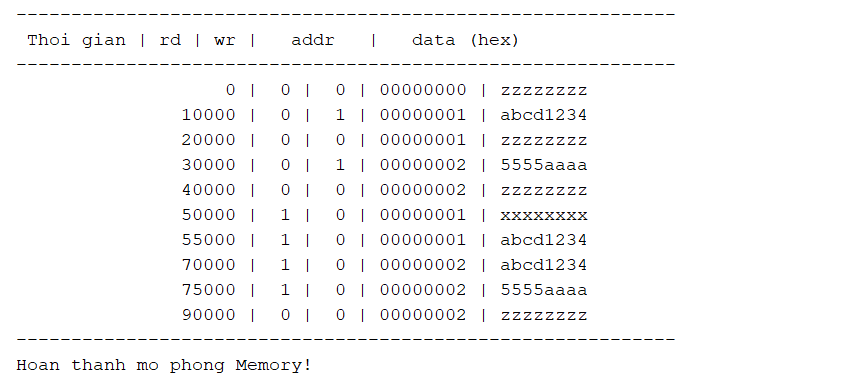
\includegraphics[width=0.8\textwidth]{consolemem.png} 
    \caption{Kết quả Console mô phỏng khối Memory}
    \label{fig:mem_console}
\end{figure}

\textbf{Đánh giá kết quả:}
\begin{itemize}
    \item \textbf{Cổng song hướng (Inout)}: Hoạt động chính xác theo cơ chế tri-state. Khi \texttt{rd=0} và \texttt{wr=0}, bus dữ liệu ở trạng thái \texttt{ZZZZZZZZ}, không gây xung đột trên đường truyền chung.
    \item \textbf{Tính đồng bộ}: Các thao tác ghi và đọc đều được kích hoạt tại cạnh lên của xung clock, đảm bảo dữ liệu được chốt vào ô nhớ và xuất ra bus ổn định, đúng nhịp hệ thống.
    \item \textbf{Độ tin cậy dữ liệu}: Kết quả đọc lại từ địa chỉ \texttt{0x01} (\texttt{ABCD\_1234}) và \texttt{0x02} (\texttt{5555\_AAAA}) hoàn toàn trùng khớp với dữ liệu đã ghi ban đầu, khẳng định mảng RAM và logic giải mã địa chỉ hoạt động đúng yêu cầu.
\end{itemize}